\section{Results}

\subsection{Ethernet Module Testing}

\subsubsection{Initial Verification}





The functionality of the Ethernet module was initially verified through a 32-bit integer transmitted from our 32-bit up-counter. This process was done to ensure the integrity of data transmission via the Ethernet interface. 

\begin{minted}{bash}
#!/bin/bash

# This script configures network interface settings for packet capturing.

# Set the path to the ethtool and ifconfig utilities
ETHTOOL=/sbin/ethtool
IFCONFIG=/sbin/ifconfig

# Define the network interface
INTERFACE=enp0s8

# Enable reception of Frame Check Sequence (FCS) for received packets
# on the network interface
$ETHTOOL -K $INTERFACE rx-fcs on

# Enable the network interface to receive all packets (including erroneous ones)
$ETHTOOL -K $INTERFACE rx-all on

# Enable promiscuous mode on the network interface to capture all network traffic
$IFCONFIG $INTERFACE promisc

# End of script
\end{minted}


The provided bash script is instrumental for network packet analysis, offering capabilities crucial for deep network traffic inspection. Here is a brief overview of its utility:

\begin{itemize}
  \item \textbf{FCS Reception:} By configuring the network interface to accept the Frame Check Sequence, the script enables detailed error analysis on incoming packets.
  \item \textbf{Receiving All Packets:} The `rx-all` setting allows for the capture of all packets, inclusive of those typically discarded, providing a comprehensive dataset for traffic analysis.
  \item \textbf{Promiscuous Mode:} Enabling promiscuous mode is key for packet sniffing, allowing the NIC to capture all network traffic, not just the traffic directed to it.
\end{itemize}





\subsubsection{Packet Analysis and Verification}
Subsequently, the accuracy of the transmitted data was validated using a Python script. This script captured the packets and verified their sequential incrementation, confirming the proper operation of the module. The Verilog simulation, illustrated in Figure \ref{fig:verilog_sim}, provides a comprehensive view of the module's behavior.

\begin{figure}[h]
    \centering
    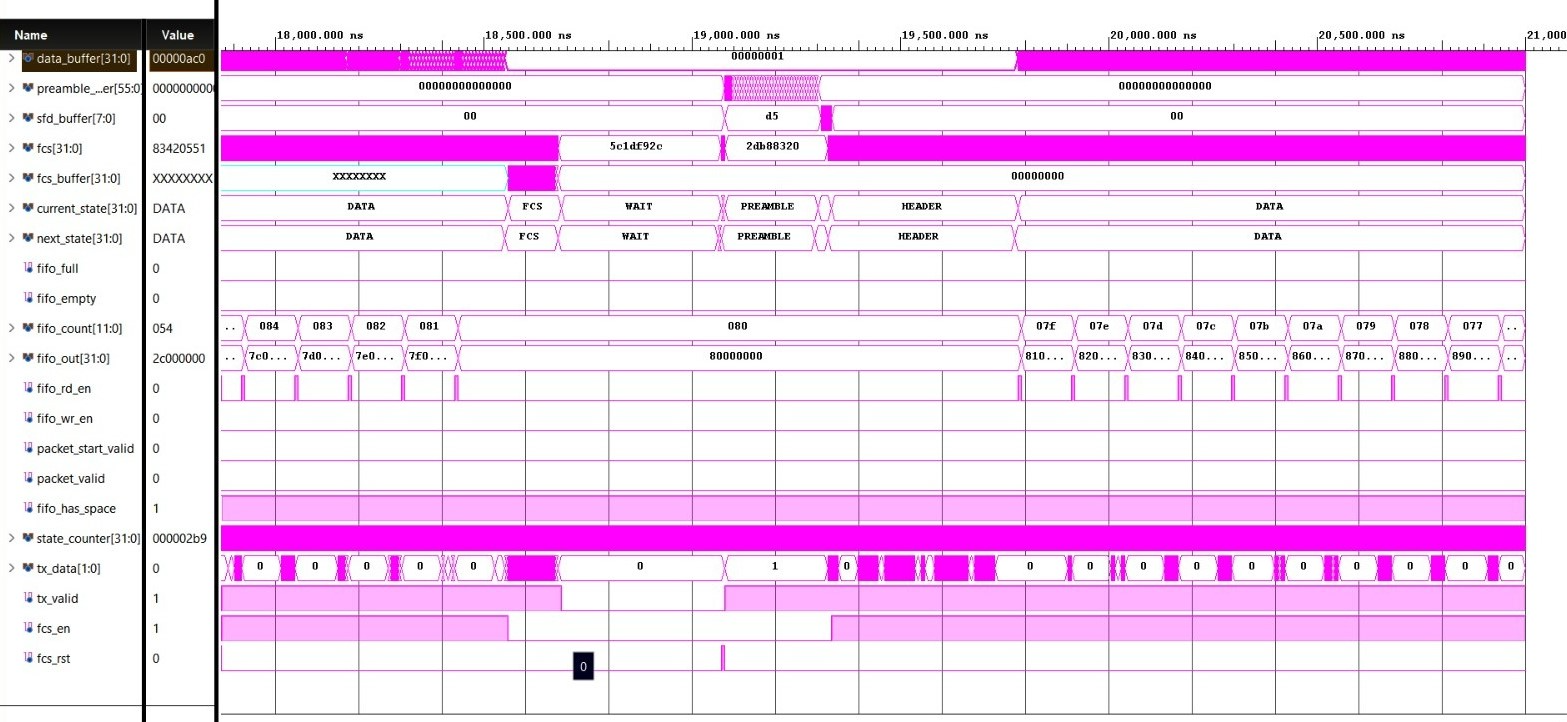
\includegraphics[width=0.95\textwidth]{Sections/RESULTS/Images/verilog_simulation.png}
    \caption{Verilog Simulation showing state transitions}
    \label{fig:verilog_sim}
\end{figure}

\subsubsection{Detailed Analysis}
A more detailed analysis is presented in Figure \ref{fig:data_payload}, where the incremental population of the data payload is visible. This figure demonstrates the consistent incrementation of the payload by a value of one.

\begin{figure}[h]
    \centering
    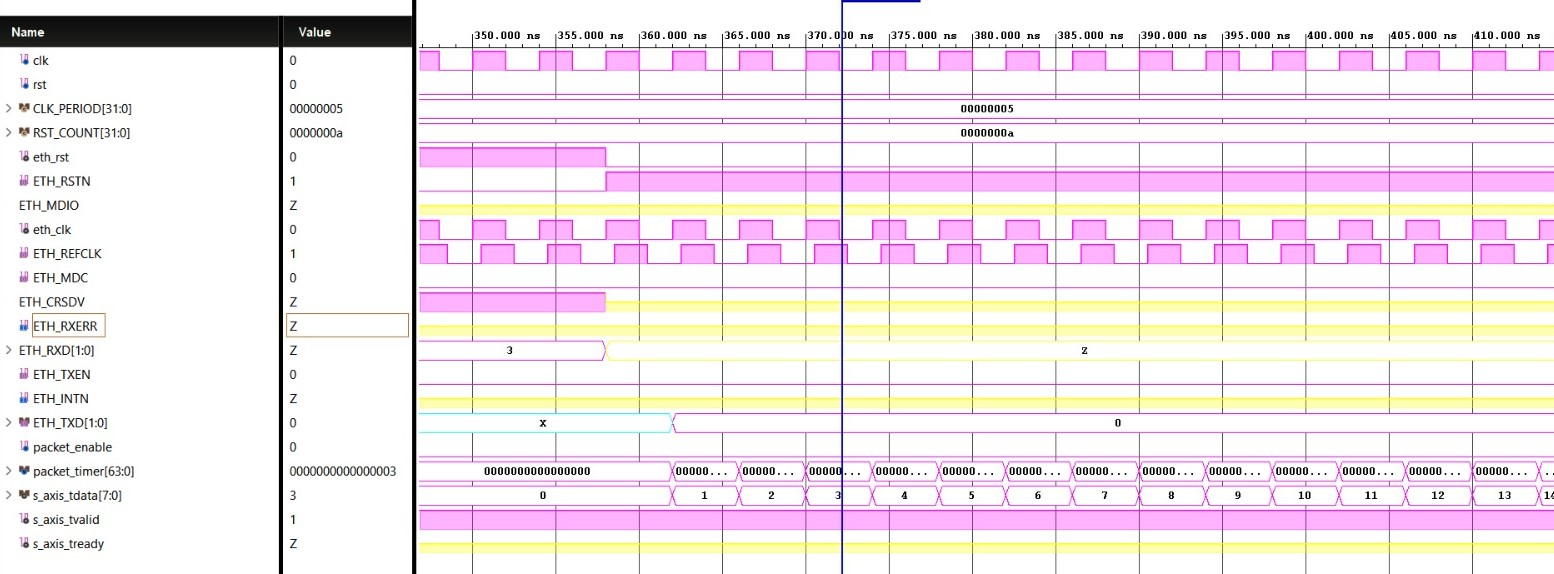
\includegraphics[width=0.95\textwidth]{Sections/RESULTS/Images/data_payload.png}
    \caption{Detailed view of data payload incrementation}
    \label{fig:data_payload}
\end{figure}

\subsubsection{Wire Shark Capture}
Lastly, Figure \ref{fig:wireshark_capture} showcases the Wire Shark capture of the packet transmission. It confirms the correct matching of source and destination MAC addresses, further validating the efficacy of our Ethernet module.

\begin{figure}[h]
    \centering
    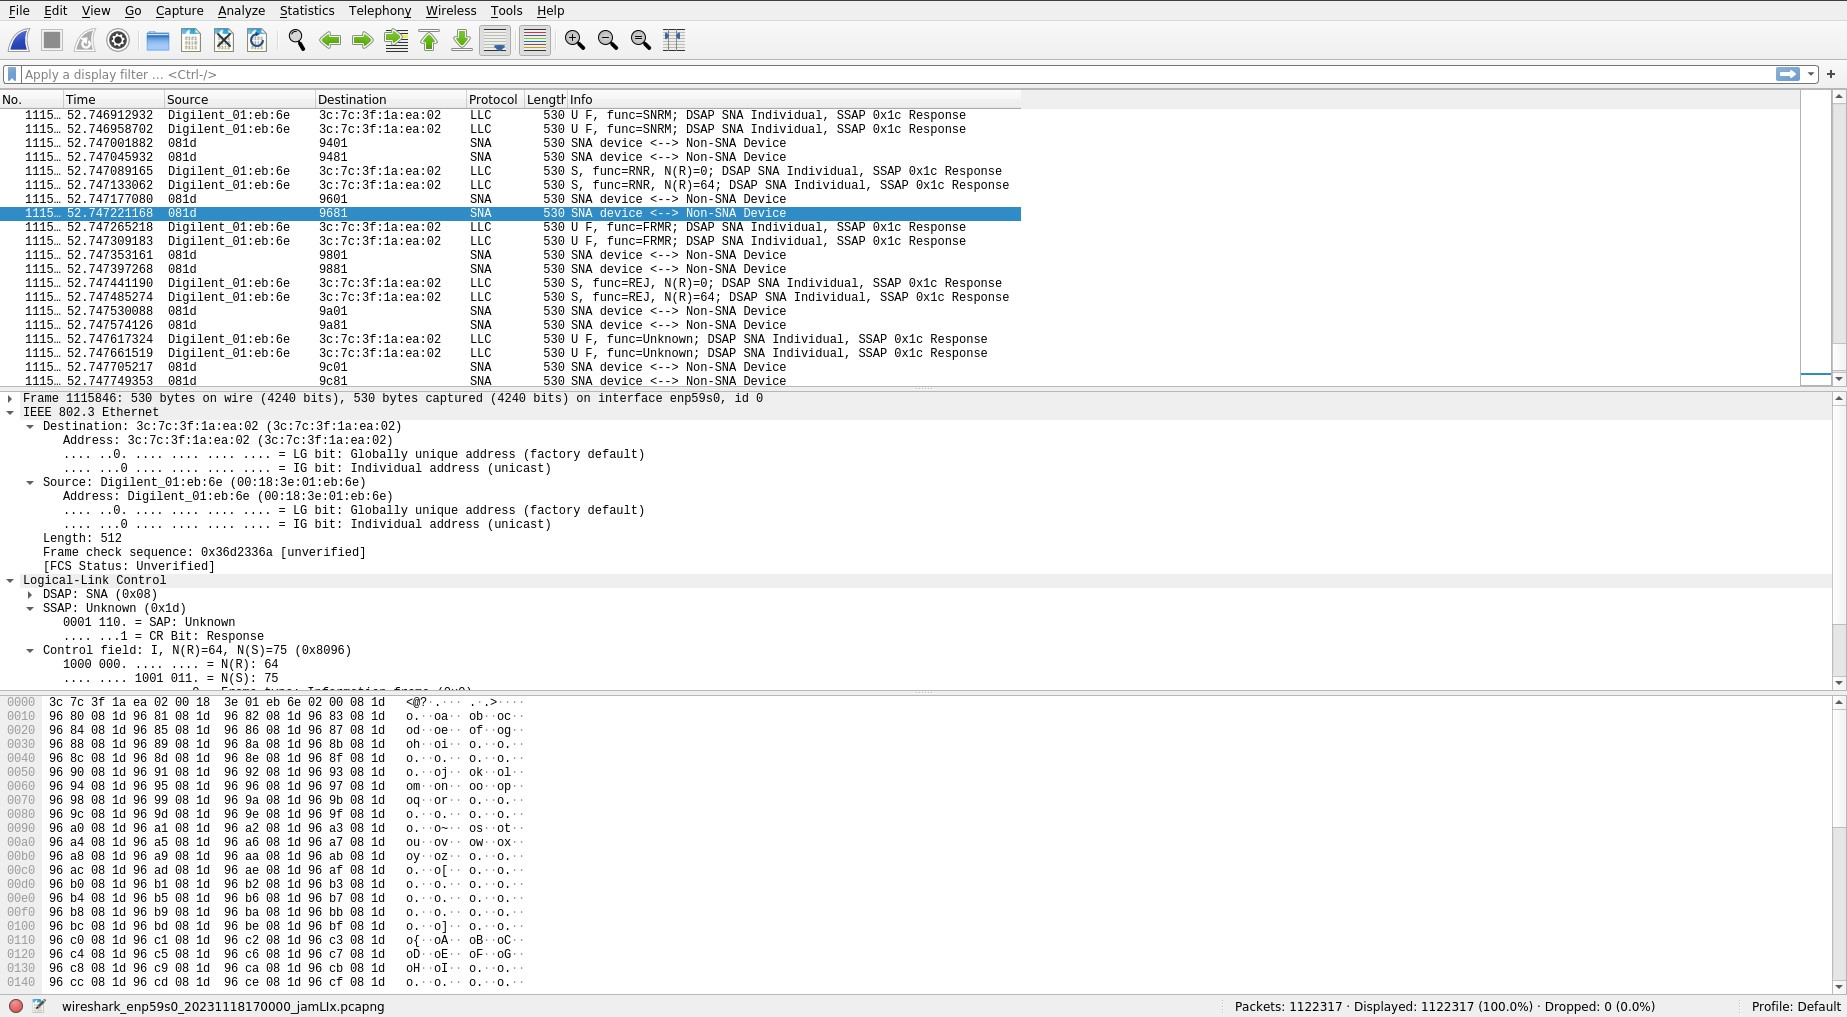
\includegraphics[width=0.95\textwidth]{Sections/RESULTS/Images/wireshark_capture.jpg}
    \caption{Wire Shark capture illustrating MAC address matching}
    \label{fig:wireshark_capture}
\end{figure}





\subsection{PDM module}




\subsubsection{LFSR and PDM Module Verification}
For the initial phase of testing the PDM module, we validated the module's operation by generating a pseudo-random sequence with a Linear Feedback Shift Register (LFSR). Figure~\ref{fig:lsfr_pdm_simulation} shows the Verilog simulation results of the LFSR and the PDM module.

\begin{figure}[h!]
\centering
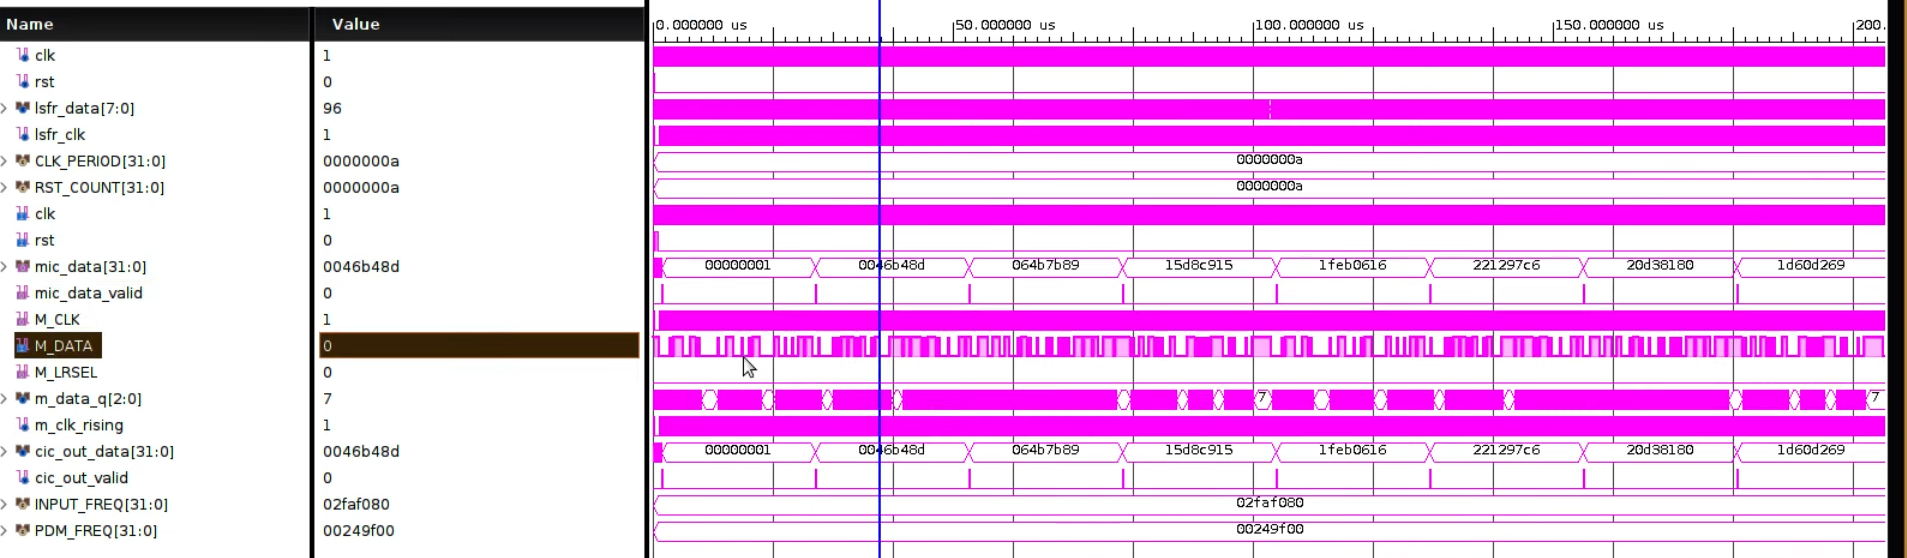
\includegraphics[width=.95\linewidth]{Sections/RESULTS/Images/verilog-tb-pdm-lsfr.png}
\caption{Verilog simulation results of the LFSR and PDM module.}
\label{fig:lsfr_pdm_simulation}
\end{figure}


\subsubsection{CIC Filter Accuracy Verification}
The accuracy of the Cascaded Integrator-Comb (CIC) filter was assessed by generating a test stimulus of a 2000 Hz sine wave, from which we derived the corresponding PDM signal. The signal was captured and stored in a test file. Figure~\ref{fig:test_stimulus_pwm_output} illustrates the input test stimulus and its Pulse Width Modulation (PWM) output form. 

\begin{figure}[h!]
\centering
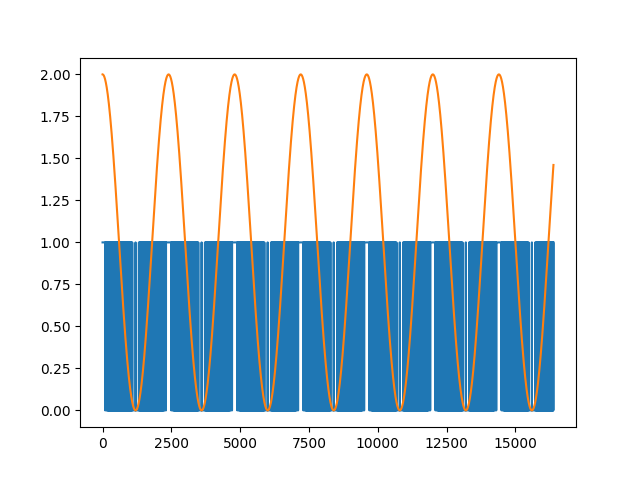
\includegraphics[width=.4\linewidth]{Sections/RESULTS/Images/PDM-Stim.png}
\caption{The generated input test stimulus and its PWM output form.}
\label{fig:test_stimulus_pwm_output}
\end{figure}

\subsubsection{Test Bench Processing}
Our test bench was configured to read the stimulus input from the provided text file and to output the processed stimulus to a separate text file. Figure~\ref{fig:cic_analog_output} depicts the analog output of the CIC filter, which appeared as a sinusoidal wave.


\begin{figure}[h!]
\centering
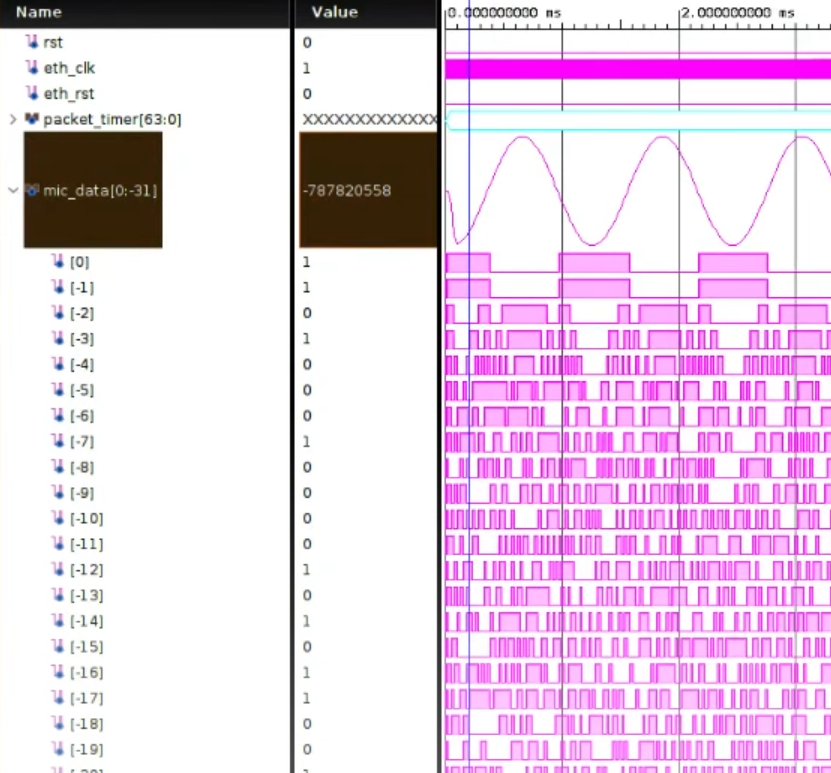
\includegraphics[width=.4\linewidth]{Sections/RESULTS/Images/verilog-tb-pdm-stim.png}
\caption{Analog output of the CIC filter.}
\label{fig:cic_analog_output}
\end{figure}

\subsubsection{Output Waveform Comparison}
To ensure the output stimulus corresponded with the expected output waveform, we utilized a Python script to plot and compare the waveforms. Figure~\ref{fig:expected_vs_actual_output} offers a juxtaposition of the expected and actual output waveforms, confirming the PDM module's performance.


\begin{figure}[h!]
\centering
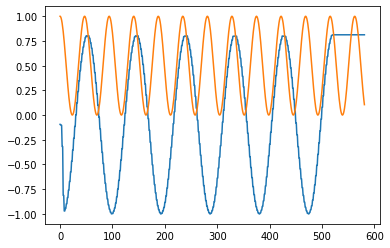
\includegraphics[width=.4\linewidth]{Sections/RESULTS/Images/exp_vs_actual.png}
\caption{Comparison of expected and actual output waveforms.}
\label{fig:expected_vs_actual_output}
\end{figure}


\subsection{Real-Time Fourier Spectrum Analysis}

The real-time Fourier spectrum of the audio signal captured by the PDM microphone is visualized on the host machine. During our demonstration, as depicted in Figure \ref{fig:fourier_spectrum}, a 1 kHz sine wave was used as the input audio. The resulting Fourier spectrum distinctly showcases peaks at the 1 kHz mark, which verifies the accuracy of the signal processing pipeline and the integrity of the captured audio signal.

\begin{figure}[htbp]
\centering
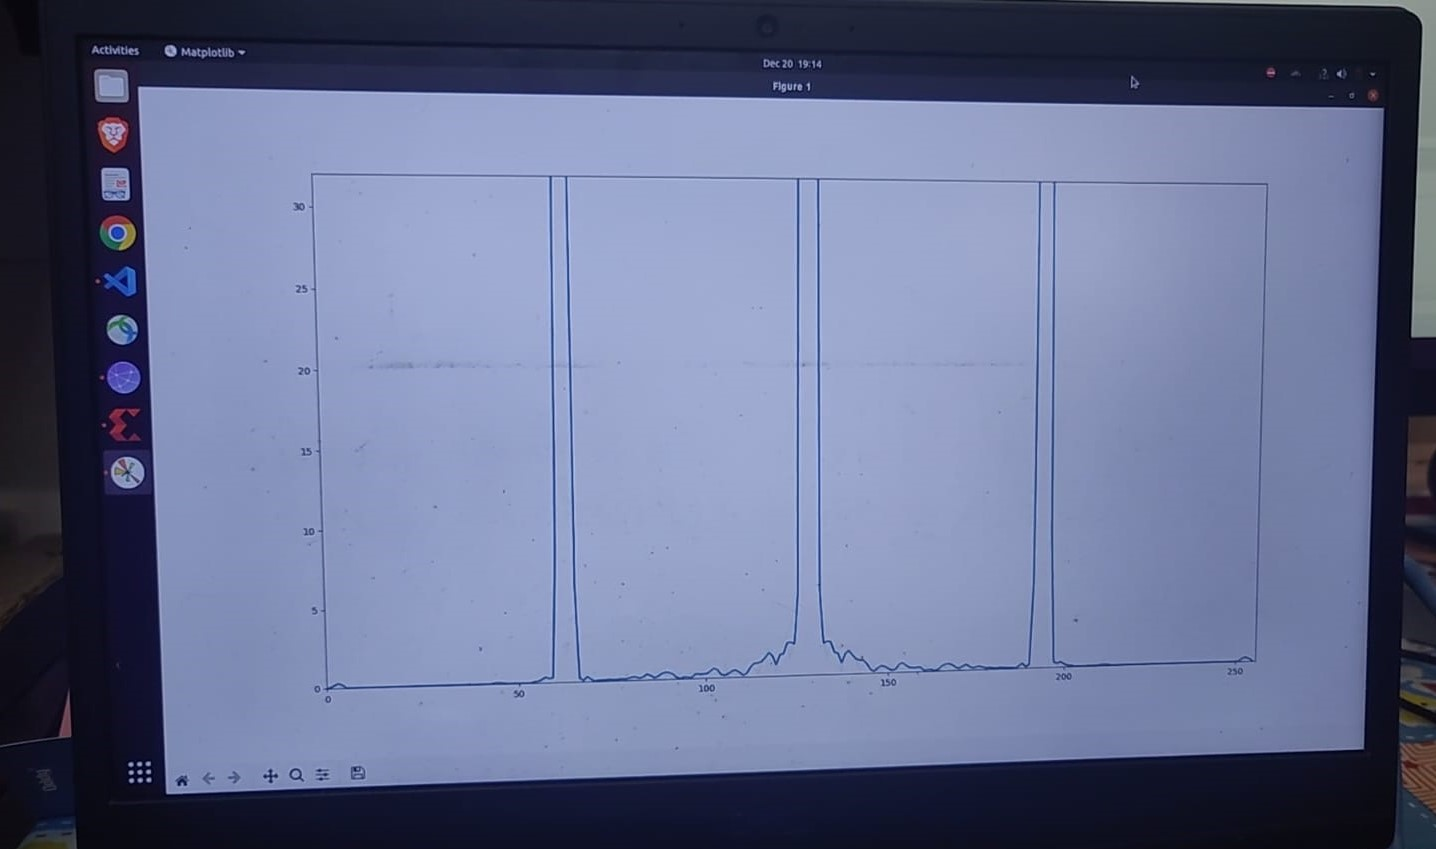
\includegraphics[width=.4\textwidth]{Sections/RESULTS/Images/realtime-fft.jpeg}
\caption{Fourier spectrum of a 1 kHz sine wave captured from the PDM microphone.}
\label{fig:fourier_spectrum}
\end{figure}



\subsection{Synthesis and Timing Report}

\subsubsection{Resource Utilization}
Figure \ref{fig:resource_util} shows the resource utilization of various modules in our FPGA design. The table indicates the usage of Look-Up Tables (LUTs), Flip-Flops (FF), Block RAM (BRAM), Ultra RAM (URAM), and Digital Signal Processing blocks (DSPs). Each module's name, the constraints applied, and the status of the synthesis are also detailed. Notably, the 'impl\_1' module has completed synthesis and bitstream generation, indicating a successful design implementation.

\begin{figure}[htbp]
\centering
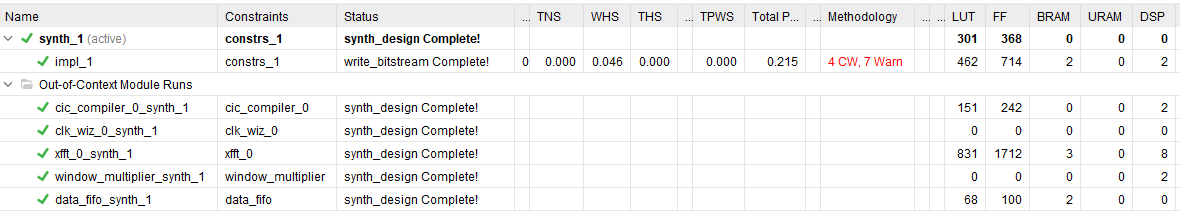
\includegraphics[width=\textwidth]{Sections/RESULTS/Images/resource-util.png}
\caption{Resource utilization summary for FPGA modules.}
\label{fig:resource_util}
\end{figure}

\subsubsection{Design Timing Summary}
Figure \ref{fig:timing_summary} presents the design timing summary. This includes the worst negative slack (WNS), total negative slack (TNS), and the number of failing endpoints for setup, hold, and pulse width conditions. The WNS of 0.541 ns for setup conditions and the worst hold slack (WHS) of 0.046 ns indicate the timing performance of the design. A zero TNS and no failing endpoints for both setup and hold suggest that the design meets the specified timing constraints.

\begin{figure}[htbp]
\centering
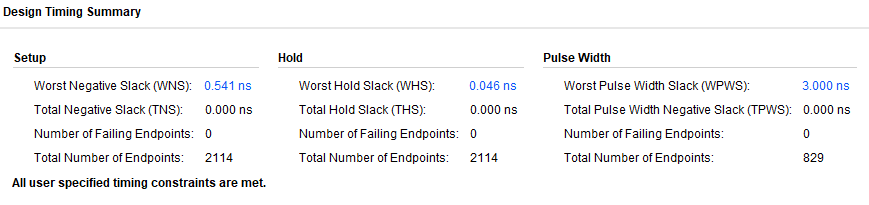
\includegraphics[width=\textwidth]{Sections/RESULTS/Images/timing.png}
\caption{Design timing summary demonstrating the setup, hold, and pulse width slack values.}
\label{fig:timing_summary}
\end{figure}
